\documentclass{eceasst}
% This is the source of the author documentation
% for the ECEASST document class.

% Required packages
% =================
\usepackage{subfig}

% Volume frontmatter
% ==================
% Volume frontmatter for OCL 2011
% =====================================
\volume{44}{2011} % Volume number and year
\volumetitle{% Title of the volume (optional)
Proceedings of the\\
Workshop on OCL and Textual Modelling\\
(OCL 2011)}
\volumeshort{% Short title of the volume (optional)
Proc.\ OCL 2011}
\guesteds{% Multiple guest editors
Jordi Cabot, Robert Clariso, Martin Gogolla, Burkhart Wolff}

% Article frontmatter
% ===================
\title{% Title of the article
Modeling the OCL Standard Library}
%\short{% Short title of the article (optional)
%Modeling the OCL Standard Library}
\author{% Authors and references to addresses
Edward Willink\autref{1}}
\institute{% Institutes with labels
\autlabel{1} \email{ed \_at\_ willink.me.uk}, \url{http://www.eclipse.org/modeling}\\
Eclipse Modeling Project}

\abstract{
OCL is widely used by UML and other languages to constrain meta-models and perform evaluations on models.
Unfortunately no OCL 2.x specification has ever been aligned with any UML 2.x specification, despite the claim of alignment at the start of the OCL specifications. The lack of alignment makes OCL's XMI interchange compliance point unachievable. This describes how introduction of an OCL pivot model may provide a solution to the alignment and a variety of other specification issues.}
\keywords{OCL, meta-model, pivot model, library, auto-generation, templates}

\begin{document}
\maketitle
\section{Introduction}

The Object Constraint Language (OCL) evolved, initially within the Unified Modeling Language (UML). As part of the UML 2.0\cite{UML-2.0} revision activities, OCL was separated out as a separate specification in recognition of OCL's utility in non-UML contexts. Unfortunately the UML Revision Task Force had insufficient resources to complete the revision of OCL 1.6\cite{OCL-1.6} to align with UML 2.0. A partially revised OCL 2.0 draft\cite{OCL-2.0-draft} was all that was available to accompany UML 2.0.

When the QVT specification was developed, the utility of OCL was recognized and OCL 2.0\cite{OCL-2.0} formed the basis for QVT 1.0\cite{QVT-1.0}. The QVT Finalization Task Force also finalized the OCL 2.0 specification, but also had insufficient resources to perform the very detailed proof reading and consistency checking for a specification involving so many cross-references.

Subsequent revisions \cite{OCL-2.2},\cite{OCL-2.3} have addressed a number of  inconsistencies, but the major problem remain unaddressed.





Each version of OCL 2.x states in its Scope statement that it is aligned with the corresponding UML 2.x specification. Sadly this statement is only an aspiration at present. Nonetheless we must proceed towards that goal and so clearly an OCL Standard Library Model should be describable by UML.

In this paper we discuss many of the issues that have arisen in building a UML-aligned meta-model for the OCL Standard Library and using that meta-model to define the Library. In a companion paper\cite{OCL-UML} we discuss issues arising from attempting to achieve UML-alignment more generally and establish the meaning of an OCL model as a combined instance of the merged UML and OCL meta-models.

It is hoped that by presenting the community with an early insight into changes that may be proposed for OCL 2.4, the community may be able to contribute constructively before, rather than after, the revised specification is adopted.

A prototype of the modeled OCL Standard Library may be found in the optional Examples and Editors of the Indigo release of Eclipse OCL, which is officially released in June 2011 and for which milestone builds have been available since December 2010. The prototype defines a Domain Specific Language to specify the OCL Standard Library, and uses Xtext tooling to provide a rich editing capability for the DSL. This facilitates entry of OCL postconditions on library operations and validates that these postconditions are consistent with the library model.

The clarifications outlined below involve very few if any, actual changes to OCL; they merely enable the specification to say what many users think it already says. Of course OCL implementations that have resolved ambiguities in alternative directions may see a change. However even changes in the specification need not impact compatibility since with substantial parts of the OCL semantics migrating to the library model, it may be possible to encapsulate the semantics of a particular OCL tool version in a corresponding OCL Standard Library model and so preserve precisely those semantics for those users that require them.

In Section \ref{LibraryUtility} we discuss the basic properties of a library model, then in Section \ref{LibraryModel} we show how a variety of OCL concepts can be captured by the library model. With a modeling capability established, in Section \ref{LibraryContent} we identify aspects of the library that deserve revision and in Section \ref{AwkwardOperations} we examine a number of operations that are difficult to model. Finally we conclude. 

\section{Background}\label{Background}

Although the OCL specification is partitioned very logically, it can appear that the specification contains more information than is necessary.

\begin{itemize}
\item Clause 7 provides a non-normative and surprisingly readable overview of OCL
\item Clause 8 specifies the Abstract Syntax: the Types and Expressions classes define the executable language, 
\item Clause 9 specifies the Concrete Syntax: the grammar and non-normative Concrete Syntax classes the define the readable language, 
\item Clause 10 specifies the Evaluation semantics: the Values and Evaluations classes define the execution behavior, 
\item Clause 11 specifies the OCL Standard Library which provides useful operations and iterations on the Types, 
\item Clause 12 specifies the Complete OCL language, an ability to define an independent OCL Document that complements a pre-existing meta-model.
\item Annex A provides a more formal but non-normative foundation for OCL semantics
\end{itemize}

The problem in understanding the specification, is that constraints that apply solely to the AST are found in Clause 8, constraints that affect construction of the AST are found in Clause 9, and constraints that affect execution of the AST are found in Clause 10, while constraints associated with specific operations are in Clause 11.

Much of Clause 10 seems very obvious and repetitious, but it serves an important, if pedantic, purpose. When dealing with operations with pre- and post-conditions, or with messages, it is necessary to be able to reason about at least two distinct system states, one before and one after a change. It is therefore necessary to fully model the system state values in order to define the semantics between two distinct sets of values.

Comparison of Clause 12 with the preceding clauses quickly reveals that Clause 12 has barely half the corresponding content; Clause 12 is still a preliminary draft, and it is in realizing Clause 12 that the major UML alignment issues arise.
 
\subsection{XMI Interchange Compliance}

The OCL specification defines a number of compliance points, of which the most important is clearly Concrete Syntax compliance. A variety of OCL tools offer a high degree of syntax interchange compliance.

The next most important is XMI compliance. No tool is able to offer more than proprietary XMI interchange, because the OCL specification omits a number of critical details and has a variety of  inconsistencies that tool implementors must use their intuition to workaround.
 
\subsubsection{OCL URI}

There is no specification of the URI of the OCL meta-model, so use of XMI from an alternative tool may require an inconvenient but comparatively simple mapping between proprietary names.

\subsubsection{OperationCallExp::referredOperation and PropertyCallExp::referredProperty}

The OCL AST refers directly to meta-model features that define operations to be invoked or properties to be accessed. The reference uses the URI of the target feature.

This can work well for user meta-models that should have stable URIs defined by the users.

Unfortunately it fails for any usage of any feature from the OCL Standard Library, since no model exists for the library as a whole and no specification of URIs is provided for the features in isolation. Tools are obliged to resort to proprietary URIs.

It also fails for any feature contributed as part of a Complete OCL document, because while Complete OCL defines features that are indistinguishable from features defined in the complemented, it is unclear how the complemented class is modified to contain the additional features and so support the URIs.

\subsection{Other Inconveniences}

\subsubsection{Iterator Operation}

The iterate and iterator operations have no UML counterpart and so cannot be represented by a UML meta-model. As a result all support for iterators requires built-in functionality, and indeed prior to OCL 2.3, the specification could be interpreted to require all names of iterators were hard-wired into the OCL grammar. OCL 2.3 clarified the status of names so that any name can be used as an iterate or iterator operation.

In our Companion paper\cite{OCLstdlib} we show how the OCL Standard Library can be defined by a model allowing arbitrary definition of operations and iterations.

\subsubsection{Complete OCL merge}

A Complete OCL document can complement a meta-model and add features to it so that they can be used as if they were part of the complemented meta-model. Additional features may be added to library types as well, so definition of an \verb|OclAny::isPersistent()| operation may add an ability to reason about the persistent storage associated with model elements.

There is no specification as to how this merged functionality is to be achieved. It is merely recognized in Clause 13.2 bullet 6 that Complete OCL supports adding features to types to which features may not be added. A convention is introduced whereby an accompanying class instance is provided for such types.

This is an uncomfortable workaround for the lack of UML alignment. It causes difficulties for tools since features are no longer defined in just one place, so the default functionality of a generic modeling framework such as Ecore must be adjusted so that all functionality that can see the meta-model features also see the accompanying class instance features. Achieving this consistently for reflective functionality is perhaps impossible since any attempt to access the container of the accompanying class instance will discover that is  an accompaniment.    

\subsubsection{OclAny conformance}

OCL uses the conformsTo relationship between types to determine substitutability. This relationship is almost identical to UML generalization; the main difference being the definition that all UML classes conform to OclAny.

Direct realisation of the above leads to some practical difficulties. Firstly the lookup of matching features must use one algorithm to traverse the generalization hierarchy, and another to extend on to OclAny. This irregularity becomes more of a concern when considering a UML operation such as \verb|Classifier::conformsTo()| which traverses the generalization hierarchy and so requires that OclAny is part of the generalization hierarchy.

\subsubsection{Reflection}

The \verb|OclAny::oclType()| operation was added to the OCL Standard Library when it was realized that the MOF \verb|Element::getMetaClass()| operation was not accessible for UML meta-models, which do not merge MOF.

Since OCL mandates that all types conform to OclAny, the availablility of \verb|OclAny::oclType()| means that all types at all meta-levels must conform to OclAny.   

\section{Analysis}

UML defines a rich suite of capabilities suitable for meta-modeling.

EMOF reduces the capabilities close to the minimum necessary to support effective use of models at run-time.

The operational scenario for OCL seems to have been overlooked. Neither of the above are appropriate for OCL usage.

In order to constrain UML types, OCL requires the full capabilities of UML types, but OCL does not need all the additional capabilities such as Deployments and Use Cases. The requirements of OCL are therefore less than UML.

However EMOF discards too much relevant modeling information and so OCL requires more than EMOF.

OCL also introduces facilities such as Iterations that cannot be represented by UML, so OCL also needs more than UML.

From this we can conclude that OCL represents a distinct usage scenario.

\subsection{Options}

We can accommodate these conflicting requirements in a variety of ways.

We could eliminate all non-UML facilities from OCL. OCL without Iterations would not be of much utility, so this is untenable.

We could eliminate the statement that OCL is aligned with UML. This is pretty much unthinkable given UML's dependence on OCL.

We could revise UML so that it supports the facilities that OCL requires. This is possible in principle, but hardly desirable since it may incur political difficulties and further practical difficulties in mutual alignment.

In the following sections we will therefore pursue an alternative approach whereby we re-use the constructive nature of the UML specification to select those packages that are relevant and then merge these with additional OCL packages to create a new UML-derived OCL pivot model.

With the OCL pivot model UML-derived, large parts of the model will automatically be UML-aligned, but we are able to adjust any UML well-formedness that are not applicable to OCL since the UML and OCL meta-models are distinct.

\subsection{Meta-Meta-Model Merge}

The OCL Pivot Model is a Meta-Meta-Model with respect to user models. The OCL Pivot model is derived by the package merge  shown in Figure~\ref{fig:UMLMMtoOCLMM}.

\begin{figure}
  \begin{center}
    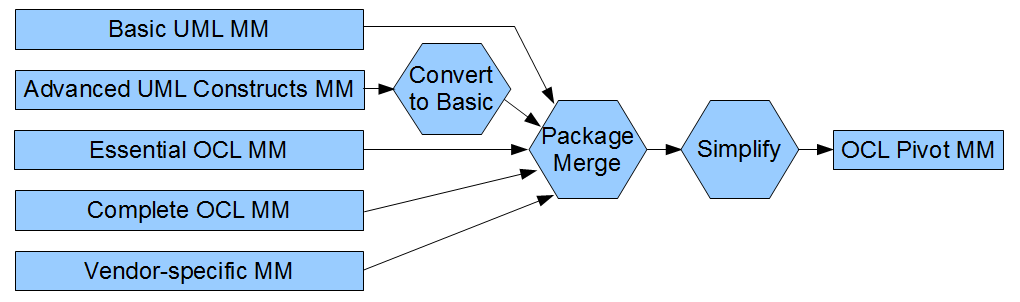
\includegraphics[width=5.75in]{UMLMMtoOCLMM.png}
  \end{center}
  \caption{Meta-Model merge to produce the OCL Pivot Meta-Model.}
  \label{fig:UMLMMtoOCLMM}
\end{figure}

The contributions to the merge are:

\subsubsection{Basic UML}

These are the UML InfrastructureLibrary::Core::Basic package that defines the Essential MOF, providing efficient but inflexible representations of each class. For instance, subset properties are eliminated so that an Operation is found in Class::ownedOperation, but not in Class::feature or Namespace::member or Namespace::ownedMember or Element::ownedElement.

\subsubsection{Additional UML}

OCL Constraint integration requires the InfrastructureLibrary::Core::Abstractions::Constraints package.

Full type support requires the InfrastructureLibrary::AuxiliaryConstructs::Templates package.

OCL Message support requires the UML::Actions::BasicActions package to define CallOperationAction and CallOperationAction. and the UML::CommonBehaviors::Communications package to define Signal.

OCL State support requires the UML::StateMachines::BehaviorStateMachines package to define State.

Unfortunately these packages were not intended to be merged into Basic, so they do not provide the same efficient representation. The Eclipse OCL prototype works around this problem by manual creation of `Basic' equivalents.

With the UML simplification process\cite{UML-simple} likely to eliminate the Basic package altogether as a primary artifact, it may be appropriate to enhance UML's QVT Operational transformation that automatically derives the Basic package to also derive basic variants of other relevant packages.

\subsubsection{Essential OCL}

These are the packages defined by Clause 8 of the current OCL specification, with minor enhancements to align with OCL. 

\subsubsection{Complete OCL}

These are the packages implied by Clause 12 of the current OCL specification, with significant revision to align with OCL. 

\subsubsection{Vendor-specific}

The package merge is not constrained to the requirements of the OCL specification. Tool vendors may merge further packages to support visitor protocols, useful operations or transient caches.

\subsection{Meta-Model Load}

Before any evaluation on a user model can occur, it's meta-model must be loaded. This currently presents challenges since users may use a variety of UML, CMOF, EMOF and Ecore dialects not all of which are supported by all tools.

Introduction of the OCL Pivot Model requires the user meta-model to be converted to, or at least interpreted in, a normalized form.

The new meta-model load phase enables the following problems to be resolved:

\begin{itemize}
\item Diverse meta-model dialects can be intermixed
\item Complete OCL documents can be represented as OCL Pivot Models
\item OCL Standard Libraries can be represented as OCL Pivot Models
\item UML generalization can be re-interpreted as OCL conformance
\item OclAny can be inserted into the conformance hierarchy
\end{itemize}

With all OCL concepts consistently modeled the OCL pivot model can be used to provide the URIs needed to solve the problem of XMI interchange.

With a normalized meta-model representation, limitations in OCL support such as navigating non-navigable associations are caused by limitations in the meta-model loader rather than in OCL.

\section{Details}

\subection{Types}

UML has distinct Type, Classifier and Classes, but OCL allows features to be added to any type eliminating the major difference between the three UML classes. All three UML classes can therefore be merged into one. The main challenge is to decide which name to use in the merged pivot model.

Of course with all types uniform, the need for companion classes to support Complete OCL operation on data types is eliminated.

\subection{EssentialOcl}
\subection{Qualified Associations}
\subection{AssociationEnd}
\subection{String...}
\subection{Values}

\section{Conclusions}

We have identified major problems in the OCL specification in regard to XMI Interchange and Complete OCL.

We have resolved these by introducing an OCL Pivot Meta-Model, and shown how this solves other problems such as UML-alignment, meta-model diversity, reflection, conformance modeling and OCL Standard Library modeling as well.

%\subsection{Manual Assembly of Bibliographies}\label{bibman}

%\noindent\textbf{To Do}

%\begin{acknowledge}
%Many thanks to Sebastian Zarnekow, Adolfo S\'anchez-Barbudo Herrera and the anonymous reviewers for helpful comments %on earlier versions of this paper.
%\end{acknowledge}

\nocite{*}
\bibliographystyle{eceasst}
\bibliography{AligningOCLandUML}

\end{document}

